\subsection{Regression Trees}

A \definition{Regression Tree} is a type of decision tree used to \textbf{predict a continuous (numeric) output variable} $Y$.

\highspace
\begin{flushleft}
    \textcolor{Green3}{\faIcon{tools} \textbf{How it works}}
\end{flushleft}
\begin{itemize}
    \item The input space (defined by predictors $X_1, X_2, \dots, X_p$) is split into \textbf{rectangular regions}.
    \item In each region, the model predicts the \textbf{mean} of the response values for the training samples that fall in that region.
    \item It forms a \textbf{piecewise-constant approximation} to the true regression function.
\end{itemize}
The splits are chosen to \textbf{minimize the prediction error}, specifically, the \textbf{Residual Sum of Squares (RSS, page \pageref{eq: RSS})}.

\begin{examplebox}[: Student Test Score Prediction]
    Imagine we have a dataset of students with:
    \begin{itemize}
        \item $X_1$: hours studied.
        \item $X_2$: sleep hours before the test.
        \item $Y$: test score (on a scale from 1 to 10).
    \end{itemize}
    We want to predict the test score using a regression tree.
    \begin{center}
        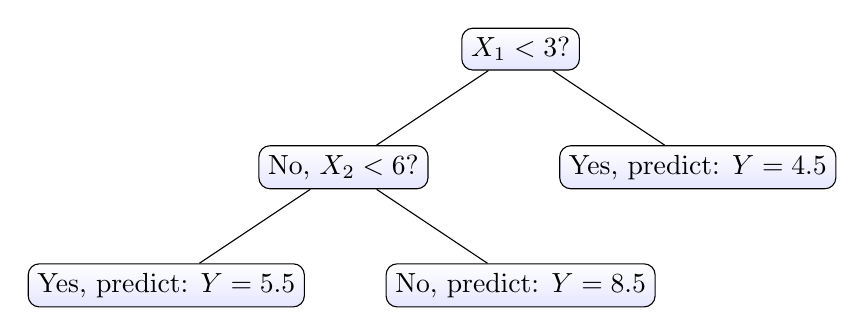
\begin{tikzpicture}[
            level 1/.style={sibling distance=45mm},
            level 2/.style={sibling distance=45mm},
            every node/.style={draw, rectangle, rounded corners, align=center, top color=white, bottom color=blue!10}
        ]

        \node {$X_1 < 3$?}
        child {
            node {No, $X_2 < 6$?}
            child {
                node {Yes, predict: $Y = 5.5$}
            }
            child {
                node {No, predict: $Y = 8.5$}
            }
        }
        child {
            node {Yes, predict: $Y = 4.5$}
        };

        \end{tikzpicture}
    \end{center}
    \begin{itemize}
        \item If a student studied less than 3 hours, predict $4.5$.
        \item If they study for at least 3 hours but sleep for fewer than 6 hours, predict $5.5$.
        \item Predict $8.5$ if they study for at least 3 hours and sleep for at least 6 hours.
    \end{itemize}
    These predictions are the \textbf{mean test scores} of students in each region of the tree.
\end{examplebox}

\begin{examplebox}[: Baseball Salary]\label{example: Baseball Salary}
    Predict a \textbf{baseball player's salary} ($Y$) based on various features ($X$), such as:
    \begin{itemize}
        \item $X_1$: number of years in the league (\texttt{Years}).
        \item $X_2$: number of hits last year (\texttt{Hits}).
    \end{itemize}
    \begin{center}
        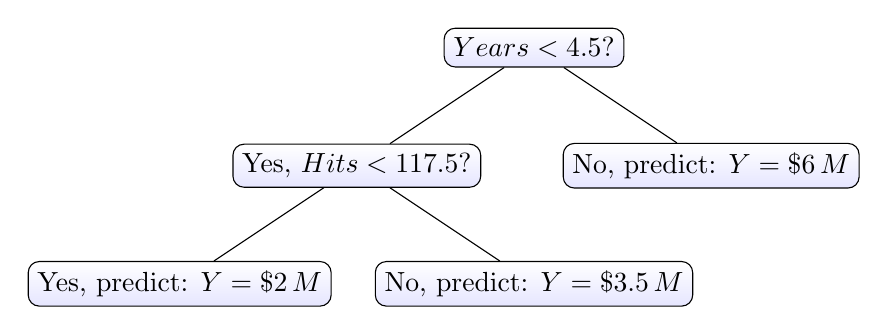
\begin{tikzpicture}[
            level 1/.style={sibling distance=45mm},
            level 2/.style={sibling distance=45mm},
            every node/.style={draw, rectangle, rounded corners, align=center, top color=white, bottom color=blue!10}
        ]

        \node {$\text{Years} < 4.5$?}
        child {
            node {Yes, $\text{Hits} < 117.5$?}
            child {
                node {Yes, predict: $Y = \$ 2\,\text{M}$}
            }
            child {
                node {No, predict: $Y = \$ 3.5\,\text{M}$}
            }
        }
        child {
            node {No, predict: $Y = \$ 6\,\text{M}$}
        };

        \end{tikzpicture}
    \end{center}
    Each \textbf{leaf node} corresponds to a \textbf{region in the (Years, Hits) space}:
    \begin{center}
        \begin{tabular}{@{} l l l @{}}
            \toprule
            Region & Condition & Salary Prediction \\
            \midrule
            R1  & $\text{Years} < 4.5$ AND $\text{Hits} < 117.5$ & $\$ 2\,\text{M}$ \\ [.5em]
            R2  & $\text{Years} < 4.5$ AND $\text{Hits} \ge 117.5$ & $\$ 3.5\,\text{M}$ \\ [.5em]
            R3  & $\text{Years} \ge 4.5$ & $\$ 6\,\text{M}$ \\
            \bottomrule
        \end{tabular}
    \end{center}
    \begin{itemize}
        \item Region R1 represents \textbf{young, less experienced} players with fewer hits, then lower salary.
        \item Region R2 represents \textbf{young but high-performing} players, then mid-range salary.
        \item Region R3 represents \textbf{veteran players}, then highest salary on average.
    \end{itemize}
\end{examplebox}